\section{Data Collection}\label{datacollection}

There are many advantages of air quality monitoring, some of which require the latency between taking a reading and it being publicly available to be as small as possible. In order to make this happen two different mechanisms can be employed. 

The first is compression of the data. This can be achieved simply by only taking measurements after a certain time has passed, or the sensor has moved by a specified amount, or both. However, with the knowledge that the data set will be sparse, compressive sampling can be performed which will allow the entire data set to be reconstructed from key readings with minimal loss of information. 

The second method is the rapid upload of data. For this to happen, the data needs to reach an access point as quickly as possible. Opportunistic uploading allows this to happen by moving data from one sensor to another in order to reach an access point rather than relying solely on the original sensor moving into range. 

\subsection{Opportunistic Uploading}\label{opportunisticuploading}

Opportunistic uploading allows a sensor, \emph{B}, to pretend to be an access point so that a sensor with data which needs to be uploaded, \emph{A}, can transfer it's data to \emph{B}. This is an advantage in that if \emph{B} meets an actual access point before \emph{A} does, the data will be transferred with less latency than it would by only using actual access points. 

\begin{figure}[H]
    \begin{center}
        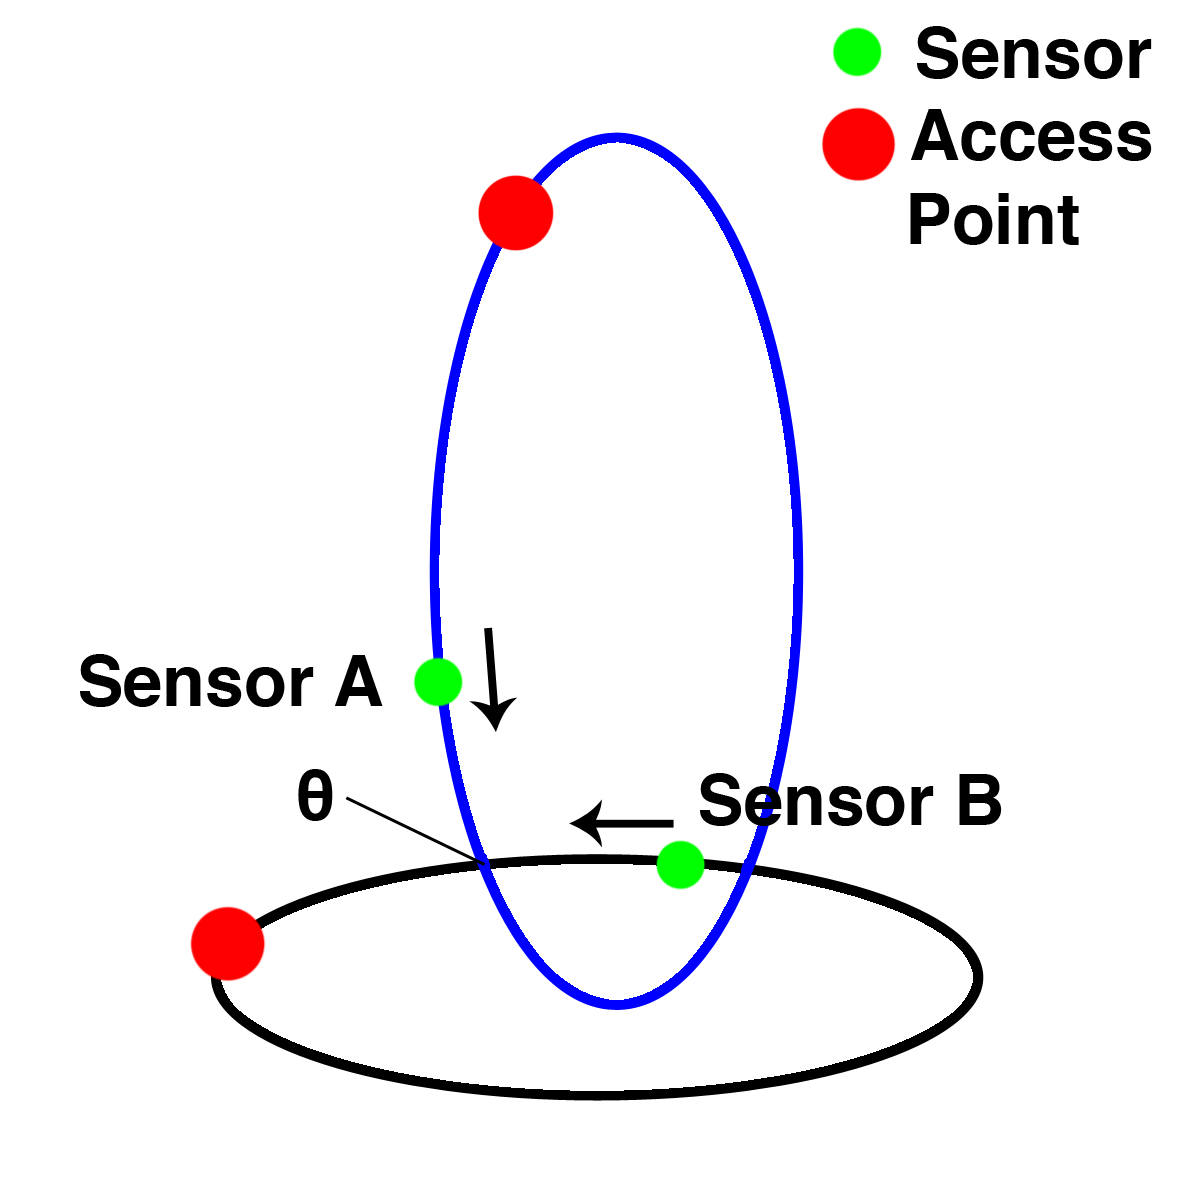
\includegraphics[scale=0.2]{./images/mpp1/Intersection.png}
        \caption{Diagram showing reduced latency. The black arrows indicated the direction of travel of the sensors. $\theta$ is the intersection point of the two routes. It can be seen that sensor A has a much further distance to travel to an access point than sensor B does.}
        \label{fig:opportunisticdiagram}
    \end{center}
\end{figure}

The situation is extremely similar to a routing protocol used in computer networks. The task is to get the information from the sensor to an access point as quickly as possible. Each link will have a certain weight associated with it and it is up to the nodes to select the appropriate route. 

Due to the predictable nature of buses, each node is capable of calculating the time it will take before it comes into range of an access point or other bus, and based on previous encounters, how long this encounter will be and therefore how much data it can upload. All this information can be used to calculate a link ``weighting'' which can be used in any standard routing protocol. 

In the case of this project the task can be simplified greatly by restricting the use of multiple hops so that data can at most move from the original sensor, to a different sensor, to the access point. This allows a single calculation to be performed to decide if data should be uploaded from \emph{A} to \emph{B}. 

There are further considerations which thought has been given to, but most require experimental results in order to answer. 

\begin{itemize}
	\item How much data should be uploaded?

		This is dependent on the upload rate of the data to the new sensor, the upload rate from the new sensor to the access point and the buffer size on the new sensor. 

	\item Which data should be uploaded?

		Older data is getting stale and applications may be waiting on it, however, it may be advantageous to provide the new data as quickly as possible as there may be time sensitive applications which do not require all data. 

	\item How often should we look for other nodes or an access point?

		If there is only access to a single wireless radio, the time a sensor spends scanning for other nodes means it spends less time listening for nodes trying to connect to it. The only solution may be to have two wireless radios. In the case of looking for the access point, this can be done by calculating the distance between the sensor and the access point using GPS data. If the distance is within a specified maximum then the sensor can start trying to connect to the access point. 

	\item Which wireless protocol is the most suitable to use for upload to the access point?

		Wifi is ubiquitous throughout the city and has high transfer rates, however it has a slow handshake. This may be crippling when sensors are only in range of each other for a few seconds at most. Bluetooth or ZigBee have much faster handshakes, but lower throughputs. This would also require dedicated access points across the city rather than simply using open access points or eduroam access points.

	\item Which wireless protocol is the most suitable to use for inter-sensor communication?

		If multiple radios are used then there is a similar situation to the above. 

\end{itemize}


Further experimentation is required with hardware to determine the average handshake length, and the average volume of data which is transferred at different relative velocities. This data can then be used to populate the parameters in the algorithm used. 




